\documentclass[10pt] {article}
\usepackage{fourier}
\author{Ankit Goyal \\ankit@cs.utexas.edu \\ CS380L}
\title{Lab 2: Networked File System}
\date{\today}	
\usepackage{full page}
\usepackage{minted} % to insert code
\renewcommand\listingscaption{Codeblock}



\usepackage{hyperref, url}
\usepackage{listings}
\usepackage{graphicx}
\usepackage{caption}
\usepackage{subcaption}
\usepackage{amsmath}
%\usepackage{amsmath, enumerate, url, ulem, algorithmic, polynom, subfig}

\setlength\parindent{0pt}

\begin{document}
\maketitle
%----------------------------------------------------------------------------------------
%  Specs
%----------------------------------------------------------------------------------------

\section{Setup}
\subsection{Hardware}

\textbf{Host 1} \\
\textbf{Processor}: 64 bit 4 core Intel(R) Xeon(R) CPU E3-1270 V2 @ 3.50GHz\\
\textbf{Memory}: 16GB \\

\textbf{Host 2: AWS micro instance} \\
\textbf{Processor}: 64 bit Intel(R) Xeon(R) CPU E5-2670 v2 @ 2.50GHz  \\
\textbf{Memory}: 1GB \\

\subsection{Software}
\textbf{Host 1 Operating System}: Ubuntu with 3.13.0-34-generic 64 bit kernel.\\
\textbf{Host 2 Operating System}: Ubuntu with 3.13.0-36-generic 64 bit kernel \\

\textbf{libssh.h} for managing ssh sessions \\
\textbf{libsftp.h} for performing file transfer \\

\textbf{NFS Server version:} Server nfs v2 Running on Host 2 \\
\textbf{NFS Client version:} Client nfs v2 Running on Host 1 \\

\textbf{FUSE version:} 30 \\


%----------------------------------------------------------------------------------------
%  Qemu Command Line
%----------------------------------------------------------------------------------------

\section{Comparison between Netfs and NFS}
\textbf{Netfs} is the network file system that I wrote for this lab and NFS is the actual network file system. My networked file system is mentioned as Netfs from now on and NFS refers to actual NFS. 

NFS server resided on a micro instance running at AWS (Host 2). Both Netfs and NFS mounted the same folder (\texttt{/home/ubuntu/shared} from Host 2) at mountdir in Host 1.

\subsection {mount time}
\textbf{NFS mount time}: 0m1.864s \\
\textbf{Netfs mount time}: 0m1.129s

Mount time for both NFS is slightly higher than the mount time of Netfs. It could be due to some network irregularities (even though I took the average). NFS mount involves RPC call to mount daemon running on server, authentication and allocating a file handle for further communication. Mount on Netfs involves setting up ssh connection and mounting the new file system locally.

\subsection {Performance Comparison}

Figure \ref{fig:thvsfair} shows the main differences between the two filesystems. In this experiment a file of 0 and 10MB (1a) are read and written back to remote disk. In Netfs initial read and write takes considerably more time when compared to NFS. Since in Netfs, we download the file first and then does local writes, subsequent writes are comparable to NFS in which writes returns only if it gets the confirmation for write. \\

\textbf{Netfs has several problems:} \\

\begin{enumerate}
  \item It will be a problem to read large files since local file system may run out of space.
  \item To start reading we need to download the file first, which introduces a huge delay to do the first read/write. 
  \item Changes won't be reflected on server if multiple clients are writing until we copy the whole file back on close.
\end{enumerate}

I tried several other experiments like writing in different chunk sizes, opening closing multiple files, writing files of different sizes, random reads in a file. In all cases NFS performed much better than Netfs. File transfer was considerably slow using \textbf{sftp} when compared to NFS and was major part of the whole transaction.

\begin{figure}[ht!]
\centering
\begin{subfigure}{.5\textwidth}
\centering
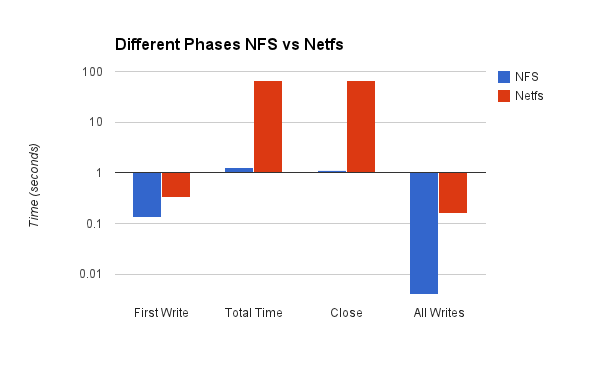
\includegraphics[width=\linewidth]{netfs1.png}
\caption{}
\label{fig:thvsfair1}
\end{subfigure}%
\begin{subfigure}{.5\textwidth}
\centering
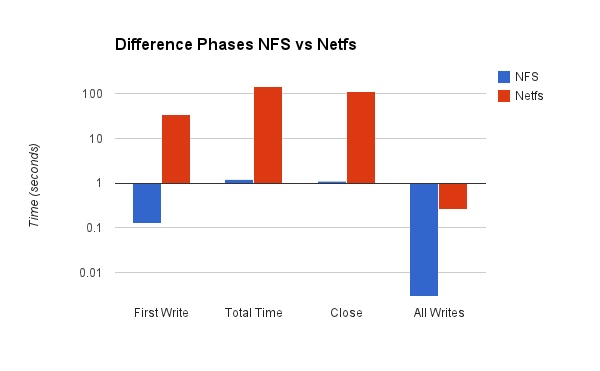
\includegraphics[width=\linewidth]{netfs2.png}
\caption{}
\label{fig:thvsfair2}
\end{subfigure}
\caption{NFS vs Netfs (a) initial file size 0 and final file size 10MB (b) initial size size 10MB and final file size 10MB}
\label{fig:thvsfair}
\end{figure}

\section {Fuse calls}
There are six major fuse calls that I implemented to get the basic functionality of networked file system. 
\subsection { \texttt{ netfs\_getattr } }
This call is equivalent to \texttt{stat} system call. It gives information about a file attributes (like mode, permissions, creation time, etc) and is essential for almost all operations. To implement this call, I use \texttt{sftp\_lstat} provided by \textbf{\texttt{libsftp}} and populate the \textbf{stbuf} buffer provided by fuse as a parameter in callback function.

\subsection { \texttt{ netfs\_readdir } }
\texttt{netfs\_readdir } returns one or more directory entries to the caller in supplied buffer. Fuse provides a \texttt{filler} function to set the contents (filenames) of the buffer. To implement this call, I used \texttt{sftp\_opendir} followed by \texttt{sftp\_readdir} to get \texttt{sftp\_attributes} structures for each file. \texttt{sftp\_attributes} contain name of the directory which can be used in filler to populate the buffer. 

\subsection{\texttt{ netfs\_open}}
\texttt{netfs\_open} opens a file. In this method, I download the requested file using \texttt{sftp\_open} followed by \texttt{sftp\_read} from remote system and store it in \texttt{/tmp}. I store the file descriptor of the tmp file in \texttt{fh} field of  \texttt{struct fuse\_file\_info} so that it can be accessed by read and write calls. 

\subsection {\texttt{netfs\_read}}
\texttt{netfs\_read} is used to read \texttt{size} bytes from file into the given \texttt{buffer} from the given \texttt{offset}. In this method, I read the file from local storage using the given parameters (offset, size) in the buffer provided by the callback function.

\subsection {\texttt{netfs\_write}}
\texttt{netfs\_write} is used to write \texttt{size} bytes into the given file. In this method, I write to the local file in \texttt{/tmp}.

\subsection {\texttt{netfs\_flush}}
\texttt{netfs\_flush} is called on \texttt{close} of file. In the call, I copy the local copy to remote server using \texttt{sftp\_write} and close the file.

\section {System Tools}

\subsection {session\_record}
\begin{listing}[ht!]
\begin{minted}{cpp}
script session_record

strace cat - > new_file

hi mom

^Dexit

\end{minted}
\label{lst:sched}
\caption{command sequence}
\end{listing}

\texttt{script} makes a typescript of terminal session. From the output it could be seen that bash first executes the cat program using \texttt{execve}. Check the permissions using \texttt{access}. Accesses several shared libraries and allocates memory. \texttt{cat} treats \texttt{-} as stdin and thus hangs to accept input from stdin. As soon as we type and hit enter, it writes the input from stdin to stdout (file descriptor 2) using \texttt{write} system call. It then again waits for input from stdin.

\subsection {\texttt{lsof | grep /dev}}
This command lists the devices  opened by different process. I see three different type of devices, \texttt{/dev/null}, \texttt{/dev/fuse} and \texttt{/dev/pts/*}. Most of the entries belong to pseudo terminals opened by \texttt{bash, vim, lsof, grep, fuse} processes.

\subsection {\texttt{tcpdump}}
I used the packet provided in the lab description, since I was on remote machine. 

\begin{listing}[ht!]
\begin{minted}{cpp}
11:19:35.188492 IP (tos 0x0, ttl 64, id 0, offset 0, flags [DF], proto UDP (17), length 328)
   128.83.158.160.68 > 128.83.158.2.67: [bad udp cksum 0x3e8f -> 0xa6f7!] BOOTP/DHCP, 
   Request from a8:20:66:3b:66:51,
   length 300, xid 0x6a228120, Flags [none] (0x0000)
	  Client-IP 128.83.158.160
	  Client-Ethernet-Address a8:20:66:3b:66:51
	  Vendor-rfc1048 Extensions
	    Magic Cookie 0x63825363
	    DHCP-Message Option 53, length 1: Release
	    Server-ID Option 54, length 4: 128.83.158.2
	    Hostname Option 12, length 7: "JUbuntu"
	    END Option 255, length 0
	    PAD Option 0, length 0, occurs 41
\end{minted}
\label{lst:sched}
\caption{Excerpt from the provided trace showing DHCP Release}
\end{listing}

DHCP messages are send over UDP. \\
Link Layer Address: \texttt{a8:20:66:3b:66:51} \\
Client IP: 128.83.158.160 \\
Server IP: 128.83.158.2 \\

In normal scenario DHCP server leases the IP address to clients and when that lease expires, it can possibly reassign that IP address to different device. Clients can renew leases to keep using the same IP, some DHCP server maintains history and try to assign same IP address to same devices. DHCP release message is sent from client to server to inform that client is finished with the address and server can reassign it to some other machine. \\

There was no acknowledgement of receipt of this message (DHCP Release) from the DHCP server. If the message is lost, server will not do anything and will let the lease expire as it normally does before assigning that IP to different device or keeping it in the pool.


\noindent \textbf{Time Spent on the lab \ensuremath{\approx} 24 hours} 

\section{References:}
1. \url{http://linux.die.net/man/2/stat}  \\
2. \url{http://api.libssh.org/master/group__libssh__sftp.html} \\
3. \url{https://github.com/ajaxorg/libssh/blob/master/include/libssh/sftp.h} \\
4. \url{http://api.libssh.org/master/libssh_tutor_guided_tour.html} \\
5. \url{http://www.cs.hmc.edu/~geoff/classes/hmc.cs135.201001/homework/fuse/fuse_doc.html}

\end{document}